% Standalone TikZ diagram: run make in this directory for PDF and SVG.
% Left: the values U_1 after one sweep. Right: the Bellman backup of (3,1).
\documentclass[11pt,tikz,border=6pt]{standalone}
% Shared style for the L11c standalone TikZ diagrams. It follows the CHEME 5820
% TikZ figures (skip-gram window, SSM block, RNN unfold): Latin Modern text,
% math labels, pastel fills with dark outlines, and plain arrows.
\usepackage[T1]{fontenc}
\usepackage{lmodern}
\usepackage{amsmath,amssymb}
\usetikzlibrary{arrows.meta,calc,positioning}
\tikzset{
  every picture/.style={font=\small},
  cell/.style={draw=black!70,line width=0.6pt,fill=white},
  goal/.style={cell,fill=green!14},
  block/.style={cell,fill=gray!30},
  focus/.style={draw=orange!70!black,line width=1.4pt,fill=orange!20},
  neighbor/.style={draw=gray!50,line width=0.6pt,dashed},
  axis/.style={draw=black!60,line width=0.5pt,-{Stealth[length=2mm]}},
  tick/.style={text=black!60,font=\footnotesize},
  note/.style={text=black!55,font=\footnotesize},
  arr/.style={-{Stealth[length=2.5mm]},thick,draw=black!75},
  chosen/.style={arr,draw=orange!70!black,line width=1.2pt},
  state/.style={circle,draw=blue!60!black,fill=blue!12,line width=0.8pt,
    minimum size=10.5mm,inner sep=0pt,font=\footnotesize},
  root/.style={state,draw=orange!70!black,fill=orange!20,line width=1.2pt},
  action/.style={circle,fill=black!80,minimum size=2.4mm,inner sep=0pt},
  prob/.style={fill=white,inner sep=1.2pt,font=\footnotesize},
}

\begin{document}
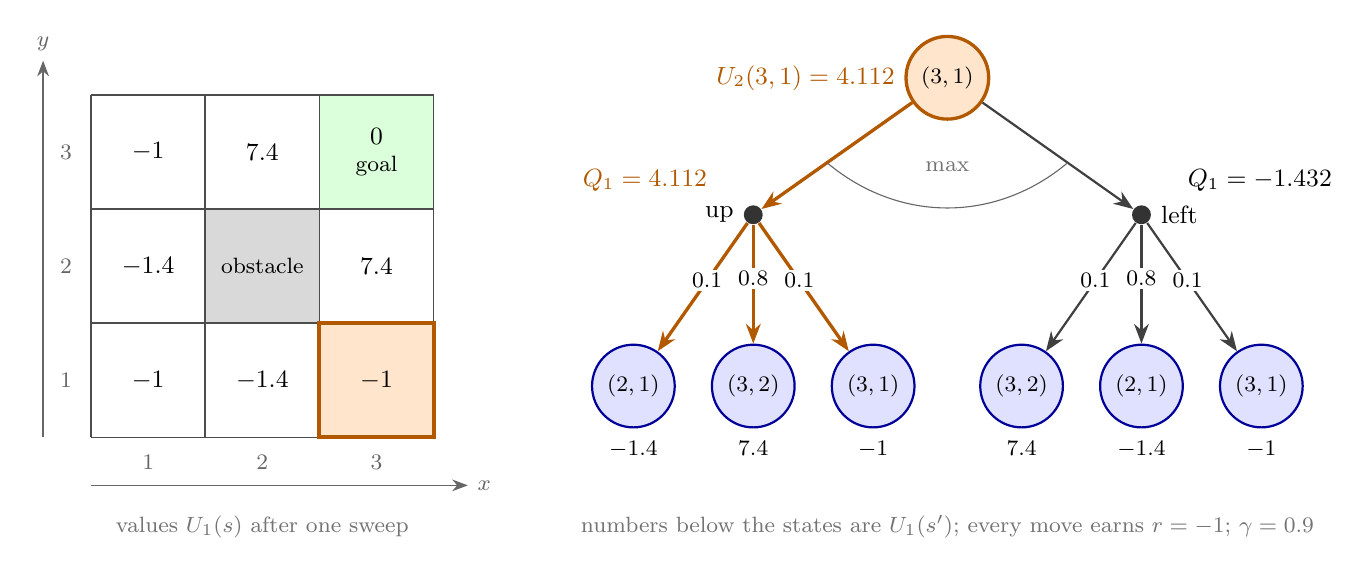
\begin{tikzpicture}[x=1.45cm,y=1.45cm]
  % --- Values after one sweep: cell (x,y) spans (x-1,y-1) to (x,y) ---
  \fill[green!14] (2,2) rectangle (3,3);
  \fill[gray!30]  (1,1) rectangle (2,2);
  \fill[orange!20] (2,0) rectangle (3,1);
  \foreach \i in {0,...,3} \draw[black!70,line width=0.6pt] (\i,0) -- (\i,3) (0,\i) -- (3,\i);
  \draw[orange!70!black,line width=1.4pt] (2,0) rectangle (3,1);
  \node at (0.5,2.5) {$-1$};
  \node at (1.5,2.5) {$7.4$};
  \node[align=center] at (2.5,2.5) {$0$\\[-1pt]{\footnotesize goal}};
  \node at (0.5,1.5) {$-1.4$};
  \node[align=center,font=\footnotesize] at (1.5,1.5) {obstacle};
  \node at (2.5,1.5) {$7.4$};
  \node at (0.5,0.5) {$-1$};
  \node at (1.5,0.5) {$-1.4$};
  \node at (2.5,0.5) {$-1$};

  \draw[axis] (0,-0.42) -- (3.3,-0.42) node[right,tick] {$x$};
  \draw[axis] (-0.42,0) -- (-0.42,3.3) node[above,tick] {$y$};
  \foreach \i in {1,2,3} {
    \node[tick] at (\i-0.5,-0.22) {$\i$};
    \node[tick] at (-0.22,\i-0.5) {$\i$};
  }
  \node[note] at (1.5,-0.78) {values $U_1(s)$ after one sweep};

  % --- Backup tree for s = (3,1): state -> action -> next state ---
  \begin{scope}[shift={(4.6,0)}]
    \node[root,label={[text=orange!70!black]left:{$U_2(3,1)=4.112$\ }}] (s) at (2.9,3.15) {$(3,1)$};
    \node[action,label={[font=\small]left:up}]    (up) at (1.2,1.95) {};
    \node[action,label={[font=\small]right:left}] (lf) at (4.6,1.95) {};
    \draw[chosen] (s) -- (up);
    \draw[arr]    (s) -- (lf);
    % max over the two actions
    \draw[black!60] ($(s)!0.62!(up)$) to[bend right=40] ($(s)!0.62!(lf)$);
    \node[note] at ($(s)+(0,-0.78)$) {max};

    % outcomes of up: slip left, intended, slip right
    \node[state] (u1) at (0.15,0.45) {$(2,1)$};
    \node[state] (u2) at (1.2,0.45)  {$(3,2)$};
    \node[state] (u3) at (2.25,0.45) {$(3,1)$};
    % outcomes of left: slip up, intended, slip down
    \node[state] (l1) at (3.55,0.45) {$(3,2)$};
    \node[state] (l2) at (4.6,0.45)  {$(2,1)$};
    \node[state] (l3) at (5.65,0.45) {$(3,1)$};

    \draw[chosen] (up) -- node[prob,pos=0.45] {$0.1$} (u1);
    \draw[chosen] (up) -- node[prob,pos=0.45] {$0.8$} (u2);
    \draw[chosen] (up) -- node[prob,pos=0.45] {$0.1$} (u3);
    \draw[arr] (lf) -- node[prob,pos=0.45] {$0.1$} (l1);
    \draw[arr] (lf) -- node[prob,pos=0.45] {$0.8$} (l2);
    \draw[arr] (lf) -- node[prob,pos=0.45] {$0.1$} (l3);

    \foreach \n/\v in {u1/-1.4,u2/7.4,u3/-1,l1/7.4,l2/-1.4,l3/-1}
      \node[font=\footnotesize,below=1pt] at (\n.south) {$\v$};

    \node[text=orange!70!black,anchor=east] at ($(up)+(-0.32,0.3)$) {$Q_1=4.112$};
    \node[anchor=west] at ($(lf)+(0.32,0.3)$) {$Q_1=-1.432$};
    \node[note] at (2.9,-0.78) {numbers below the states are $U_1(s')$; every move earns $r=-1$; $\gamma=0.9$};
  \end{scope}
\end{tikzpicture}
\end{document}
